\documentclass[10pt,twocolumn,letterpaper]{article}

\usepackage[pagenumbers]{cvpr}

% Include other packages here, before hyperref.
\usepackage{graphicx}
\usepackage{amsmath}
\usepackage{amssymb}
\usepackage{booktabs}
\usepackage{CJKutf8}
\usepackage{float}
\usepackage{minted}
\usepackage{mdframed}
\usepackage{makecell}
\usepackage{url}
\usepackage{ifthen}
\usepackage{color}
% \usepackage{epsfig}

% If you comment hyperref and then uncomment it, you should delete
% ReviewTempalte.aux before re-running LaTeX.
% (Or just hit 'q' on the first LaTeX run, let it finish, and you
%  should be clear).
% \usepackage[pagebackref,breaklinks,colorlinks]{hyperref}
\usepackage[pagebackref,breaklinks,colorlinks,bookmarks=false]{hyperref}

% \input{mysetup.tex}

% \iccvfinalcopy % *** Uncomment this line for the final submission

\def\cvprPaperID{9487} % *** Enter the CVPR Paper ID here
\def\confName{CVPR}
\def\confYear{2022}

\definecolor{red}{rgb}{0.9,0.1,0}
\definecolor{blue}{rgb}{0.4,0.4,0.9}
\definecolor{green}{rgb}{0, 0.4, 0}
\definecolor{orange}{rgb}{1, 0.5, 0}
\definecolor{purple}{rgb}{0.6, 0, 0.6}
\definecolor{darkgreen}{rgb}{0, 0.4, 0.4} 

\newboolean{revising}
\setboolean{revising}{true}
\ifthenelse{\boolean{revising}}
{
    \newcommand{\jordan}[1]{\textcolor{green}{jordan:#1}}
    \newcommand{\frank}[1]{\textcolor{blue}{frank:#1}}
    \newcommand{\lysee}[1]{\textcolor{orange}{13:#1}}
    \newcommand{\leo}[1]{\textcolor{purple}{leo:#1}}
    \newcommand{\yz}[1]{\textcolor{darkgreen}{yz:#1}}
    \newcommand{\TODO}[1]{\textcolor{red}{todo:#1}}

} {
    \newcommand{\TODO}[1]{#1}
    \newcommand{\jordan}[1]{{#1}}
    \newcommand{\frank}[1]{{#1}}
    \newcommand{\lysee}[1]{{#1}}
    \newcommand{\leo}[1]{{#1}}
    \newcommand{\yz}[1]{{#1}}
}

% \newcommand{\shouldcite}{\TODO{[X]} }


\begin{document}

%%%%%%%%% TITLE
\title{An Interesting Fighting Game using Style-based Generative Adversarial Network and Real-time Human Pose Estimation (Final)}

\author{Lin-Yung Hsieh\\
National Tsing Hua University\\
{\tt\small s111061553@m111.nthu.edu.tw}
% For a paper whose authors are all at the same institution,
% omit the following lines up until the closing ``}''.
% Additional authors and addresses can be added with ``\and'',
% just like the second author.
% To save space, use either the email address or home page, not both
\and
Jin-Cheng Jhang\\
National Tsing Hua University\\
{\tt\small s111061540@m111.nthu.edu.tw}
\and
Yu-Cheng Hsieh\\
National Tsing Hua University\\
{\tt\small s111061517@m111.nthu.edu.tw}
\and
Yi-Shan Lee\\
National Tsing Hua University\\
{\tt\small s110061623@m110.nthu.edu.tw}
\and
You-Ze Huang\\
National Tsing Hua University\\
{\tt\small s111033545s@m111.nthu.edu.tw}
}

\maketitle


%------------------------------------------------------------------------

\begin{abstract}
short summary of the project with main results
\cite{lugaresi2019mediapipe}
\end{abstract}

\section{Introduction}
% introduce the problem you want to solve, expain why it is important to solve it; and indicate the method you used to solve it. add a concept figure showing the overall idea behind the method you are presenting.
We want to implement a 2-people fighting game. When entering the game, two players will take a selfie respectively as their player avatar in the game. During the game, the camera will capture the players' human pose, reflecting the human pose in the game. When the player raises his/her right hand, for example, the avatar will go right.

Besides, as a player is attacked in the game, the face of avatar (we call it source face) will gradually change into another face (target face). The more health points a player loses, the more his/her avatar will change. The player should try his/her best in order to keep his/her face from turning into other people's face.
\section{Related Work}
% Sec 2.1. Review of previous work (i.e. previous methods that have explored a similar problem)
% Sec 2.2. Say why your method is better than previous work; and/or summarize the key main contributions of your work;
\subsection{StyleGAN}
When it comes to generating images from style aware latent codes, StyleGAN-based work must first come to our mind. There are several styleGAN based works, such as original styleGAN \cite{karras2019style} and styleGAN2 \cite{karras2020analyzing}. These works focus on diversity and quality on the generated images. However, the ultimate goal of these works is using random latent code to generate diverse and plausible images, while our goal is to use specific latent code to reconstruct the same images and apply latent code interpolation to mix the style of two given faces, which is totally different from original styleGAN based works.

To address this issue, we finally find some similar works called style encoding. Style encoding generates corresponding latent codes based on input images. We find two works focusing on style encoding tasks \cite{karras2020training} \cite{richardson2021encoding}. Finally we decide the latter one because its style encoder outperforms the former one. 

\subsection{Human Pose}
There are many existing work focusing on human pose estimation, such as YOLO \cite{yolo1} \cite{wang2022yolov7} \cite{yolo3}. However, we find that if we inference on our laptop, it'll run very slow. The FPS of the game will drop to 2 or 3, which is unsuitable for our application. What we need is a simple backbone that can perform human pose estimation real-time, instead of a heavy backbone that can predict very accurately.

Therefore, we search for a simple network that satisfies our goal, \textbf{mediapipe}~\cite{lugaresi2019mediapipe}. We find that it can perform human pose estimation in real-time, mainly due to two reasons. First, Figure~\ref{fig:yolo_arch} and Figure~\ref{fig:mp_arch} shows the architecture of YOLOv7~\cite{wang2022yolov7} and mediapipe respectively. We can easily find that the architecture of YOLOv7~\cite{wang2022yolov7} is far more complicated than that of mediapipe~\cite{lugaresi2019mediapipe}, which implies that the number of parameters in mediapipe~\cite{lugaresi2019mediapipe} is far less than that in YOLOv7~\cite{lugaresi2019mediapipe}, so the inference speed will be faster.

\begin{figure}[ht]
    \centering
    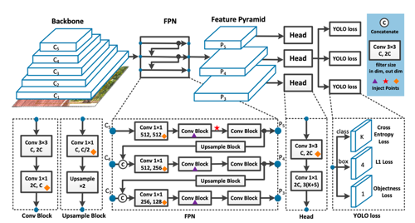
\includegraphics[scale=.6]{fig/yolo_arch.png}
    \caption{Architecture of YOLOv7 \cite{wang2022yolov7}.}
    \label{fig:yolo_arch}
\end{figure}

\begin{figure}[ht]
    \centering
    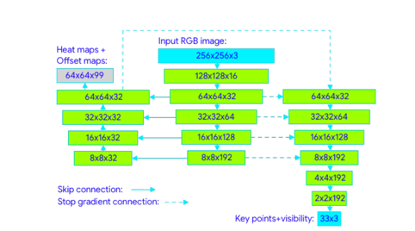
\includegraphics[scale=.6]{fig/mp_arch.png}
    \caption{Architecture of Mediapipe \cite{lugaresi2019mediapipe}.}
    \label{fig:mp_arch}
\end{figure}

Second, unlike most human pose backbones that perform detection at every single frame, mediapipe only performs human detection at the very beginning frame as Figure \ref{fig:mp_det} shows. This approach greatly reduces the computational cost. Combined with 2 advantages mentioned above, mediapipe seems to be the best choice for our application.

\begin{figure}[ht]
    \centering
    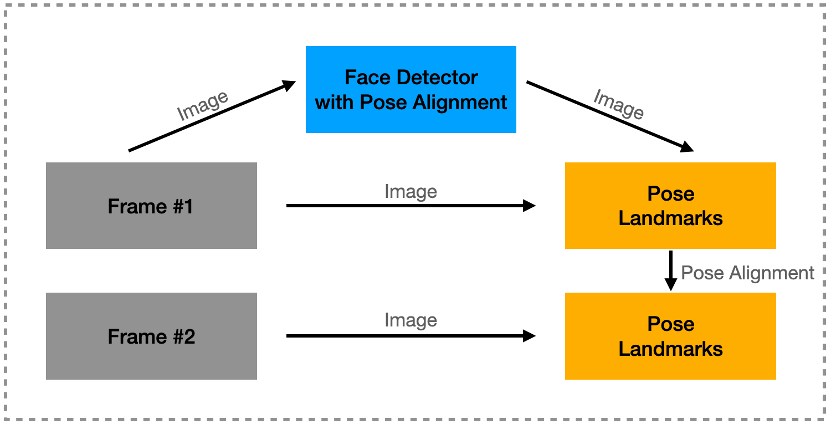
\includegraphics[scale=.5]{fig/mp_det.png}
    \caption{Mediapipe only performs human detection at the very beginning frame, which greatly reduces the computational cost.}
    \label{fig:mp_det}
\end{figure}

The original version of mediapipe, however, only supports human pose estimation for single person, but our game definitely requires the simultaneous huamn pose estimation on two people. Therefore, we make some modifications to it, which will be elaborated in Section \ref{mediapipework}.
\section{Technical Part}
% Sec 3.1: Technical part: Summary of the technical solution
% Sec 3.2: Technical part: Details of the technical solution; you may want to decompose this section into several subsections; add figures to help your explanation.

% \begin{figure*}[h]
    \begin{center}
        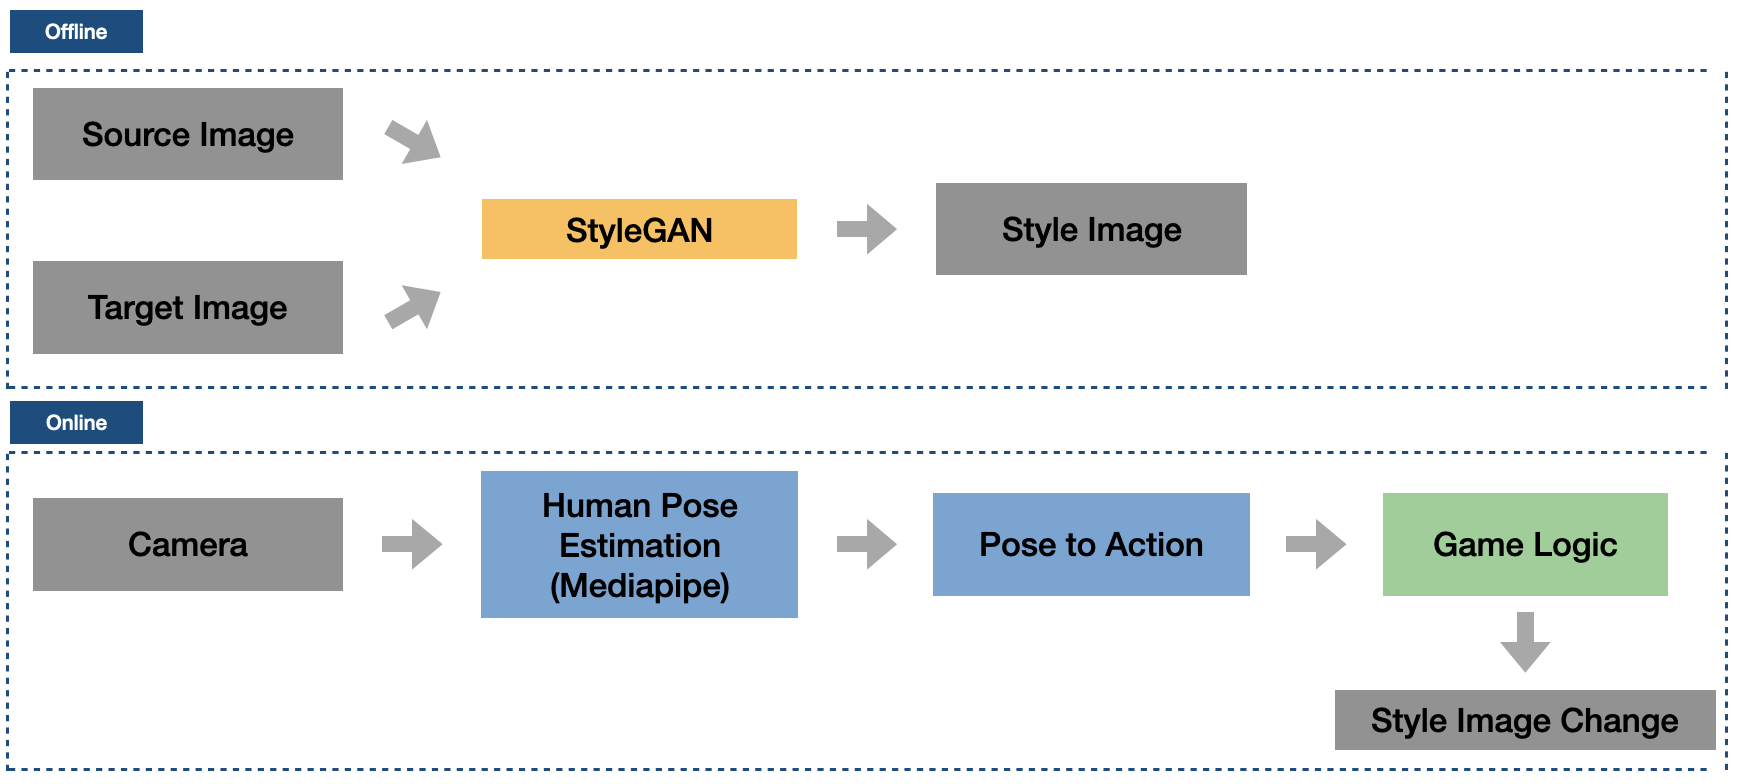
\includegraphics[width=1.0\linewidth]{fig/cv_framework.png}
    \end{center}
    \caption{\textbf{System flow chart} Players will take a selfie respectively as their player avatar before the game starts. During the game, the camera will capture the players’ human pose, reflecting the human pose in the game. The faces in the game will also change by time according to the health points of each player.
    }
    \label{fig:framework}
\end{figure*}
In this section, we present the framework for our game, which is depicted in Figure~\ref{fig:framework}. There are methods of detailed implementation.

%-------------------------------------------------------------------------
\subsection{StyleGAN} \label{StyleGAN}
In order to mix the style of two real faces, we utilize the style encoding~\cite{richardson2021encoding}, style mixing, latent code interpolation and StyleGAN~\cite{karras2019style} \cite{karras2020analyzing} inference. Firstly, Style encoding aims to find a corresponding latent code $w$ from a real image $I$ such that the generated image $I'$ from $w$ is very similar to the original real image $I$ (you can regard this task as a reconstruction task). We use Style encoder to transform source images $I_{source}$ and target image $I_{source}$ to obtain corresponding latent vectors $w_{source}$ and $w_{target}$ and then use these latent vectors to do latent code interpolation.
our style encoder architecture are shown in Figure~\ref{fig:styleEncoder}.



Secondly, the main idea of latent code interpolation is to get a sequence of latent codes $[w_1,...,w_n]$ by interpolating different proportion of latent code $w_{source}$ and $w_{target}$, where $n$ is the length of sequence (e.g. $w_1$ consists of 95\% of $w_{source}$ and 5\% of $w_{target}$ ; $w_2$ consists of 90\% of $w_{source}$ and 10\% of $w_{target}$...)

Finally, we will put results from latent code interpolation $[w_1,...,w_n]$ into StyleGAN model and the model outputs a sequence of images $[I_1,...,I_n]$ that mixed the style of $w_{source}$ and $w_{target}$. From the left part of the sequence $I_1,I_2,...$ preserves more information of $w_{source}$ while the right part of the sequence $I_n,I_{n-1},...$ preserves more information of $w_{target}$. In our game, we will change the player's face base on image sequences $[I_{source},I_1,I_2, ... ,I_n,I_{target}]$ whenever the player loses health points. 

\begin{figure*}[ht]
    \centering
    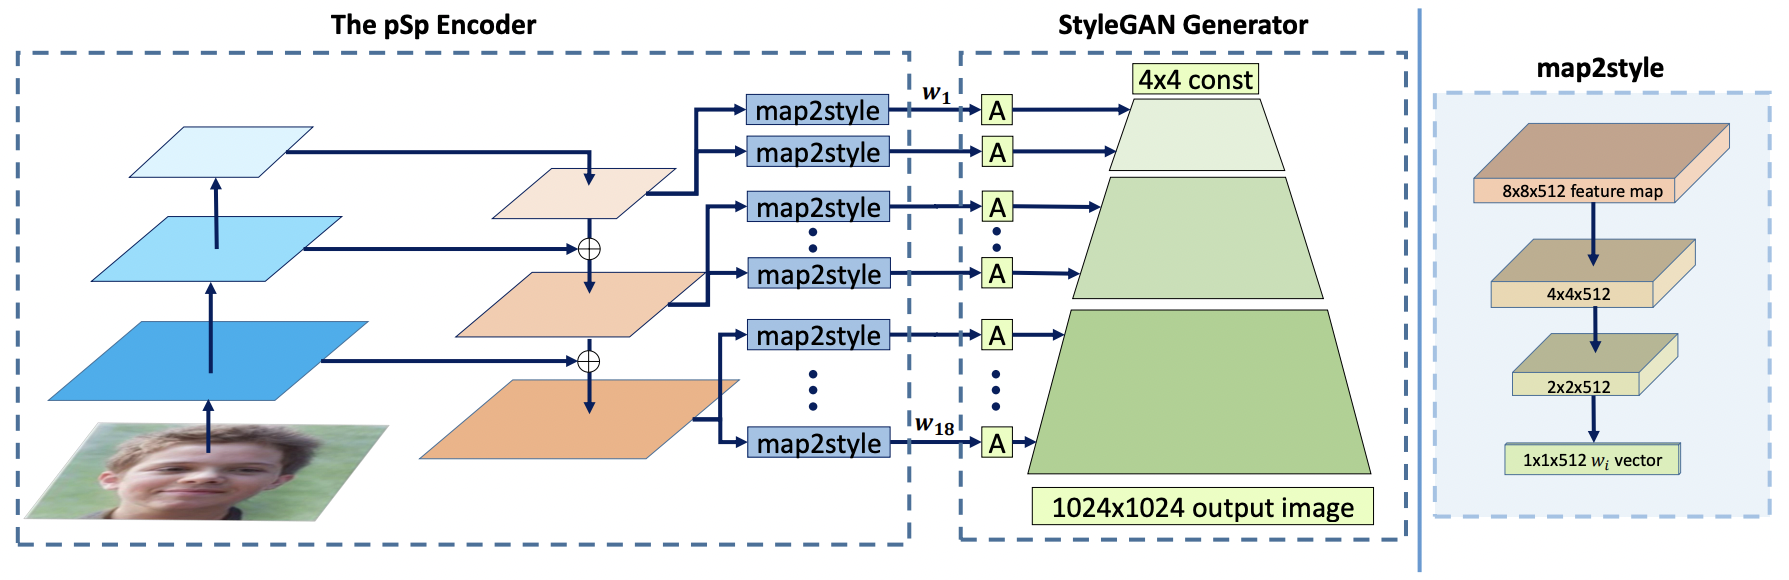
\includegraphics[scale=.5]{fig/pixel2style2pixel_pipeline.png}
    \caption{Style Encoder architecture}
    \label{fig:styleEncoder}
\end{figure*}


\subsection{Human pose estimation} \label{HPE}

In order to reflect the human action in the game, we need a model that can predict real-time human pose. Besides, due to the immediacy we require in our game and the laptop we use without the high Compute Capability GPU, the model cannot be too computationally expensive. Therefore, we discard some state-of-the-art human pose estimation frameworks such as YOLOv7~\cite{wang2022yolov7}. 

\label{mediapipework}
Instead, we select \textbf{mediapipe}~\cite{lugaresi2019mediapipe} developed by \textbf{Google} to achieve real-time human pose estimation. It captures the real-time image from the camera and performs real-time single person human pose estimation, which can predict 33 key points as Figure~\ref{fig:medpose} shows.

In order to predict two people's key points in one image, we crop the image into two halves. One person stands on the left side and the other stands on the right side. We perform their pose estimation individually. The position matrix of the left-side person is denoted as $M_{left}=[[x_1, y_1],[x_2, y_2],...,[x_{33}, y_{33}]]$ and the position matrix of the right-side person is denoted as $M_{right}=[[x_1, y_1],[x_2, y_2],...,[x_{33}, y_{33}]]$, where $x$ and $y$ are the positions of each key point. We can use these 33 key points to predict actions such as "raise right hand." Take "raising right hand" for example. When the position $y$ of key point 15, the right wrist, is larger than the position $y$ of key point 0, the nose, we can define the action as "raising right hand." This is how the pose-to-action step work.


\begin{figure}[ht]
    \centering
    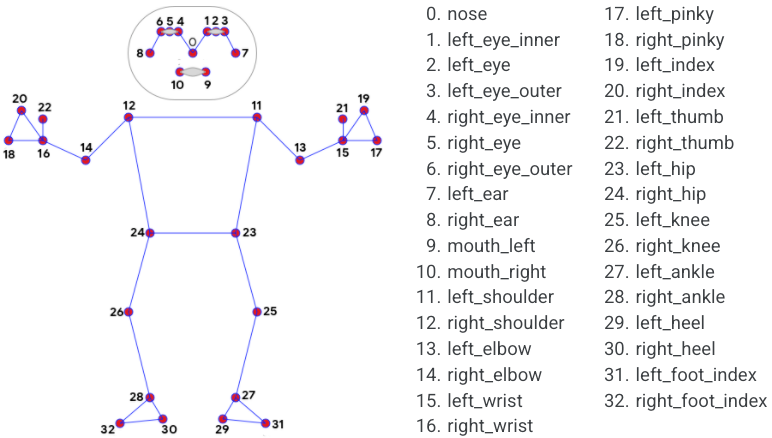
\includegraphics[scale=.3]{fig/medpose.png}
    \caption{33 key points predicted by mediapipe~\cite{lugaresi2019mediapipe}.}
    \label{fig:medpose}
\end{figure}


%-------------------------------------------------------------------------
\subsection{Game interface}
In this part, we will need to create the GUI of this game.
Besides, it is important to integrate the StyleGAN \ref{StyleGAN} and  human pose estimation \ref{HPE} into this game.

% At the beginning of the game, two players will first take a selfie through the camera, and the pictures will become the faces of the characters in the game and show on the screen. Next, when the game starts, we will receive the real-time actions from the previous part of human pose estimation (Sec. 2.2), then the game characters will do the corresponding actions on the screen.

% Throughout this game, whenever the character is attacked, his/her health point will drop. Meanwhile, we will switch his/her face to the next image which comes from the sequence of the player's style images (Sec. 2.1). The game will come to the end if one of the character's face completely become the pre-selected target image, in another words, the health point equals to zero.

\subsubsection{Basic GUI}

We use \texttt{pygame} module to implement this game and the main framework is refer to \cite{GUI_framework}. In the game GUI shown in Figure \ref{fig:gui}, we have several features such as health bar, background, music, character, etc. Two players can use keyboard to control the actions of the game characters. The actions include move, jump, attack, and defense. When the character is being attack, his health point will minus 10. However, if the character successfully defend the attack, the health point will only drop by 2. Both the attack and the defense have a cool-down time for 1 second. Whenever the health drops to zero, the game will terminate and restart a new match.

\begin{figure*}[ht]
    \centering
    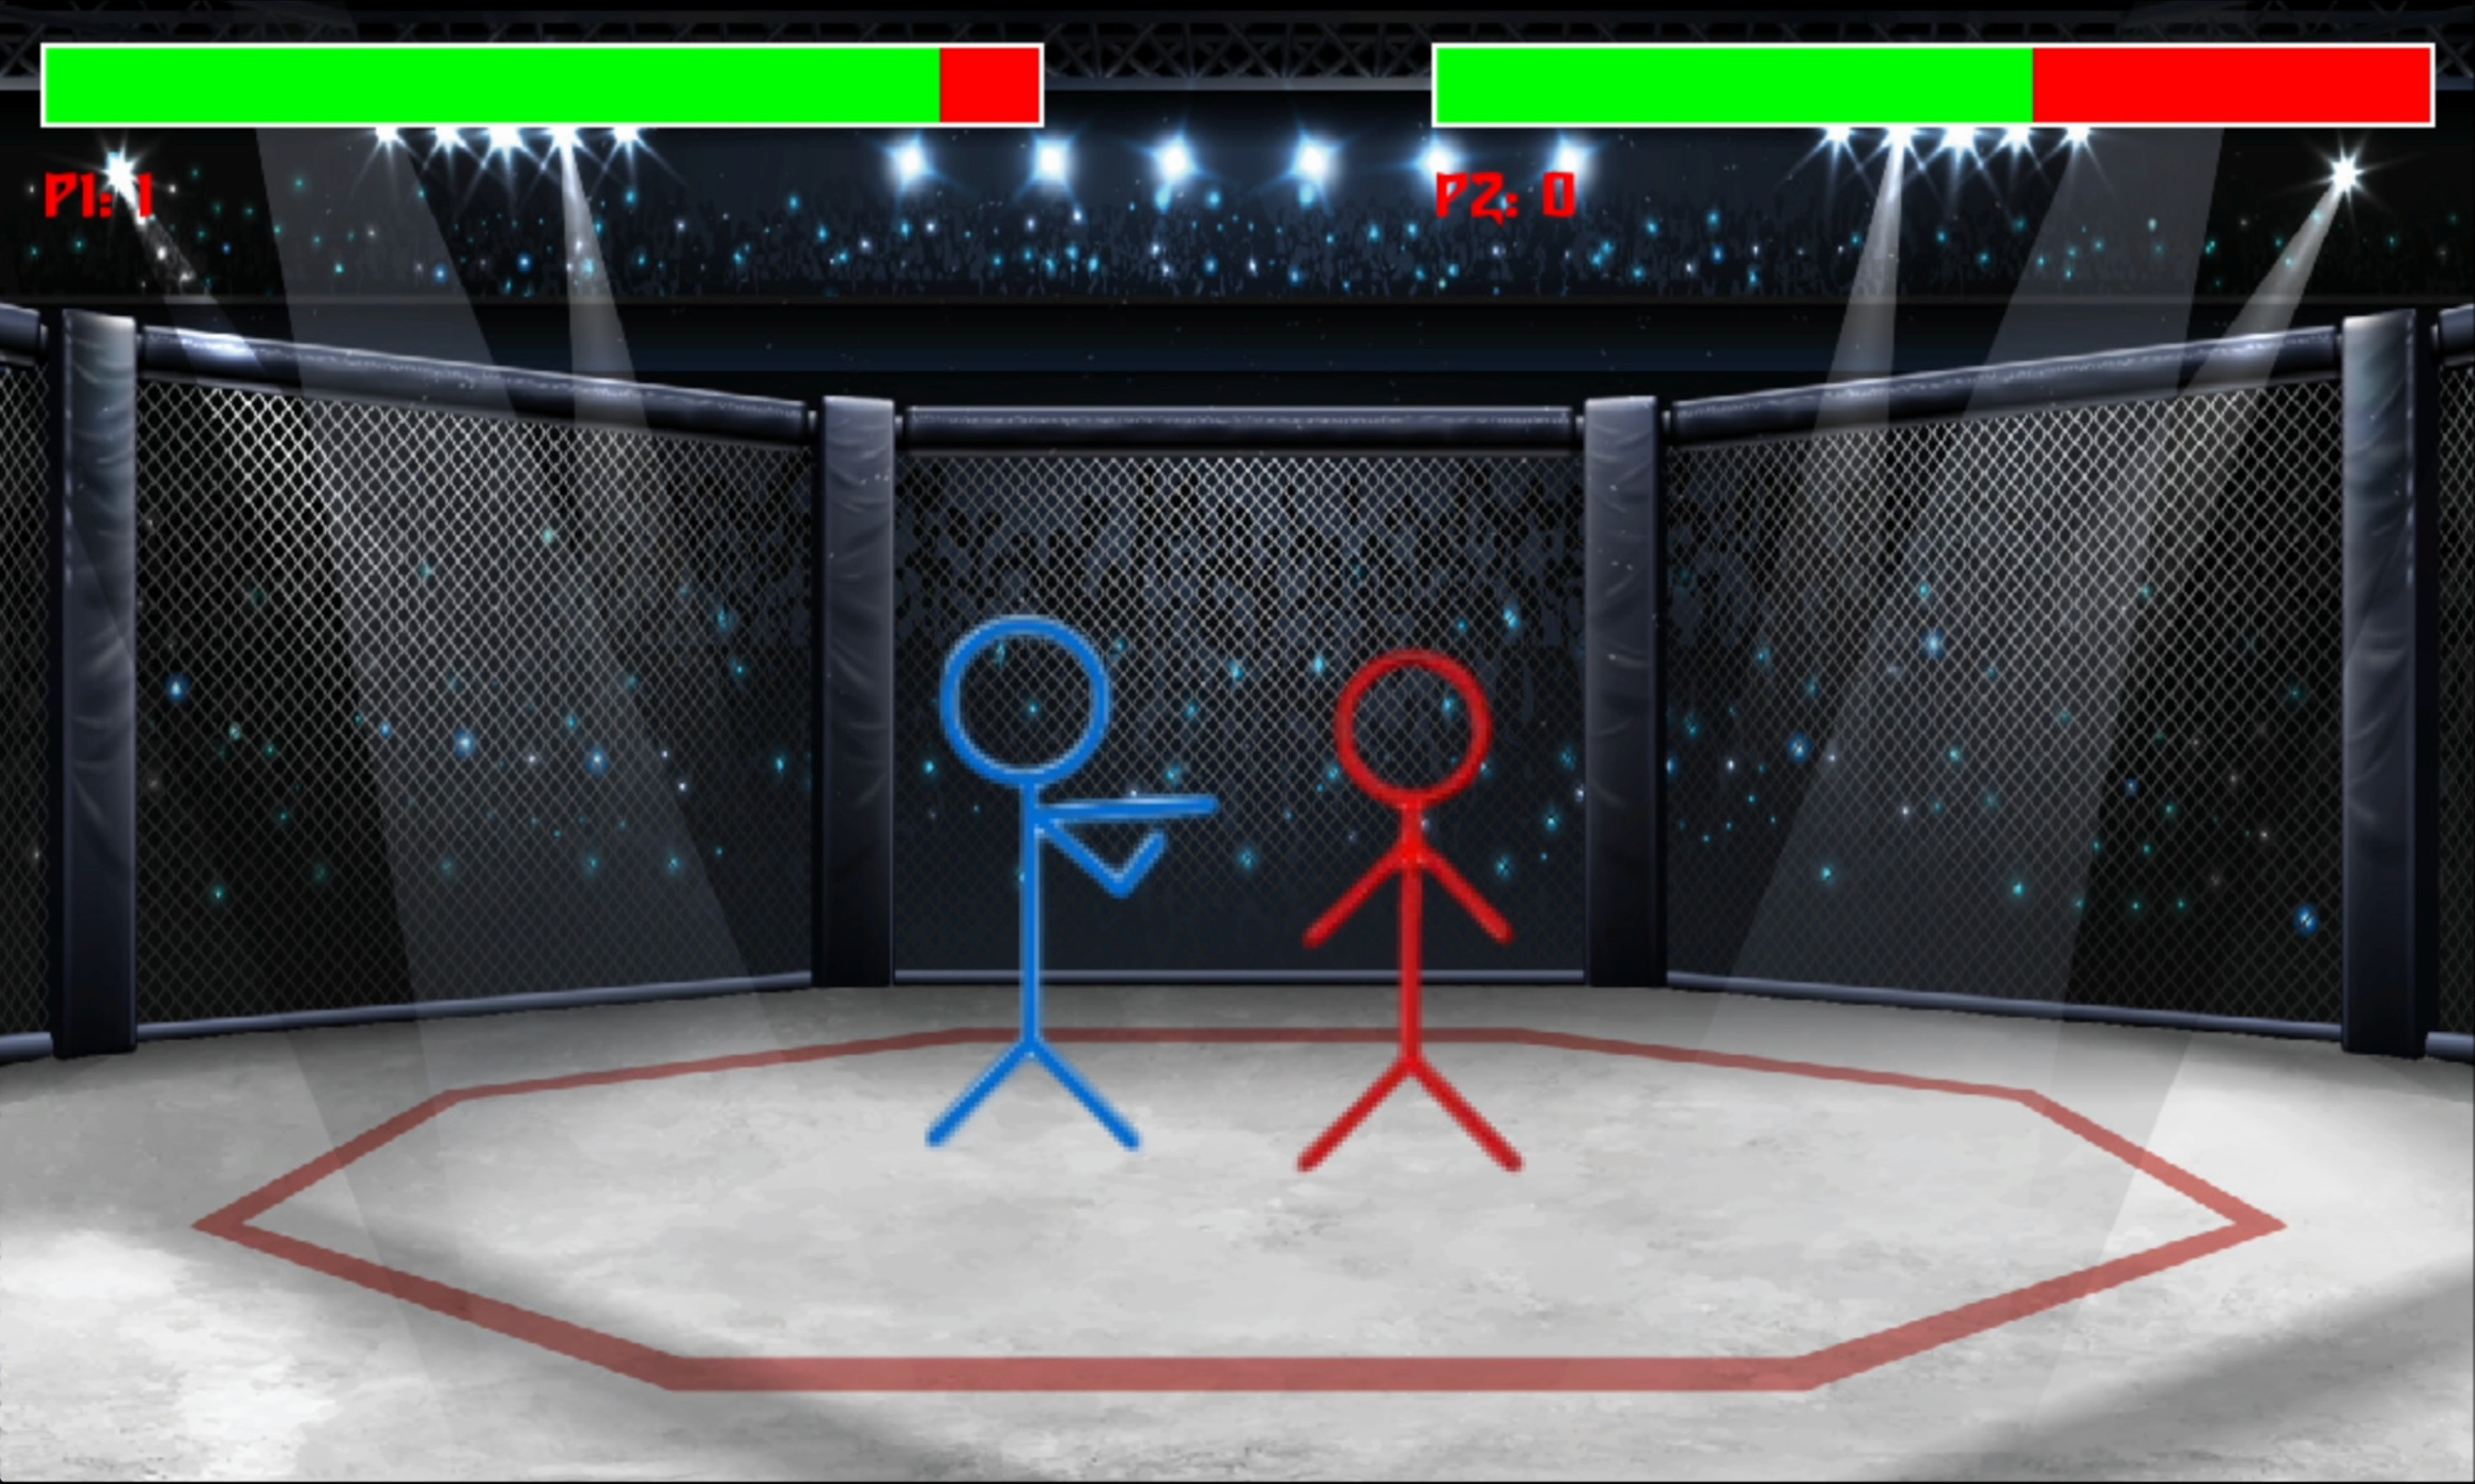
\includegraphics[scale=.1]{fig/game_gui.jpg}
    \caption{GUI of our fighting game}
    \label{fig:gui}
\end{figure*}
\subsubsection{Sprite}

In order to let the game characters do an action on the screen, we drew a stickman sprite shown in Figure \ref{fig:sprite} on our own. In the sprite, each row represents an action. For example, the fifth row stands for "attack". When the player presses the attack button on the keyboard, the image in the fifth row will sequentially change from the first frame to the last frame rapidly. Therefore, we can see the attack action showing on the GUI.

\begin{figure}[ht]
    \centering
    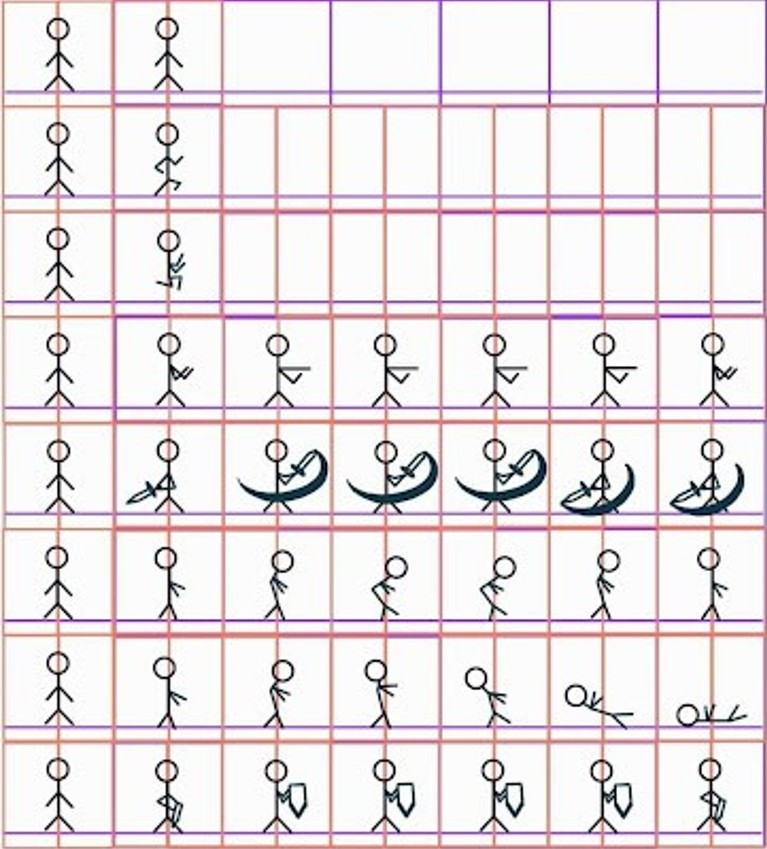
\includegraphics[scale=.35]{fig/sprite.jpg}
    \caption{Sprite for animation}
    \label{fig:sprite}
\end{figure}

\subsubsection{Integration with human pose estimation}

In this part, we need to replace the original keyboard input with the result from the human pose estimation. For the implementation detail, the actions come from the players will be stored in a boolean list and sent to a function in the game interface. When any element of the list equals to True, we will regard it as the same meaning of having a keyboard input. In this way, we can successfully integrate with the human pose estimation.

\subsubsection{Integration with StyleGAN}
Before the game starts, we will receive a sequence of style images pre-calculated by StyleGAN. With these images, we will sequentially put them on the game character's face. Throughout this game, whenever the health point of the character drop by 10, the image will switch to the next one. Therefore, we achieve the effect that the game character's face will gradually change from the player's selfie to the target image.
% the above things have to be place here, or all titles will compromise  --Jordan

\section{Experiment}

\subsection{StyleGAN}
In this section, we will present the result of the style fusion of the source image and target image in Figure \ref{fig:source target image}. The fusion image is present in Figure \ref{fig:stylechange}. According to this result, there are several points that we can discuss.

As shown in Figure \ref{fig:stylechange}, the style interpolation of the reconstructed source image and the reconstructed target image is very successful. We can actually see the hairstyle, faces and background of the reconstructed source image gradually fuse into those of the reconstructed target image with smoothness. The result proves that interpolation of latent code in latent space actually leads to style fusion of image space.

According to Figure \ref{fig:source target image} and \ref{fig:stylechange}, the reconstruction of the source image and the target image is quite a failure. After some discussion, we find out some points that may lead to this undesirable result. These points are listed below:

\subsubsection {Face position problem}
During implementation, we find that the whole reconstructed image will change greatly if we slightly scale the original image. Figure~\ref{fig:face position problem} can fully explain this problem. We divide the four images in Figure~\ref{fig:face position problem} into two groups. The leftmost two pictures are one group, and the rightmost two pictures are another group. Both groups of image contains original image(left one) and reconstructed image(right one). The two images of left part of Figure~\ref{fig:face position problem} is the same as left part of Figure \ref{fig:source target image} and upper left of Figure~\ref{fig:stylechange}. We just cut a little fraction below the neck on the original image Figure \ref{fig:source target image}, the reconstructed image varies a lot (shown in right part of Figure~\ref{fig:face position problem}). 

To be more specific, compared to the reconstructed image that does not cut, the reconstructed image has more hair and wrinkles. The hair and wrinkles, however, have nothing to do with the neck (cut place). We attribute this result to the fact that GAN-based models are inherently very hard to control the generated results.

\subsubsection {Origin goal problem}
The main goal of StyleGAN-based model is to generate diverse results using latent code, while our goal is to reconstruct original image using latent code, which is totally opposite. This might be a potential reason of our bad result.

\subsubsection {Domain gap problem}
The style encoder is trained on FFHQ dataset, which consists mostly of Caucasian and African. Our source and target images are both Asian, which may lead to a domain gap problem.

\subsubsection {Latent code space problem}
Losing information is inevitable when encoding the high dimensional images to low dimension latent vectors. Thus, we will lose considerable information when we perform style encoding. As a result, StyleGAN generator cannot generate images similar to original images.


\begin{figure}[ht]
\centering
    \centering
    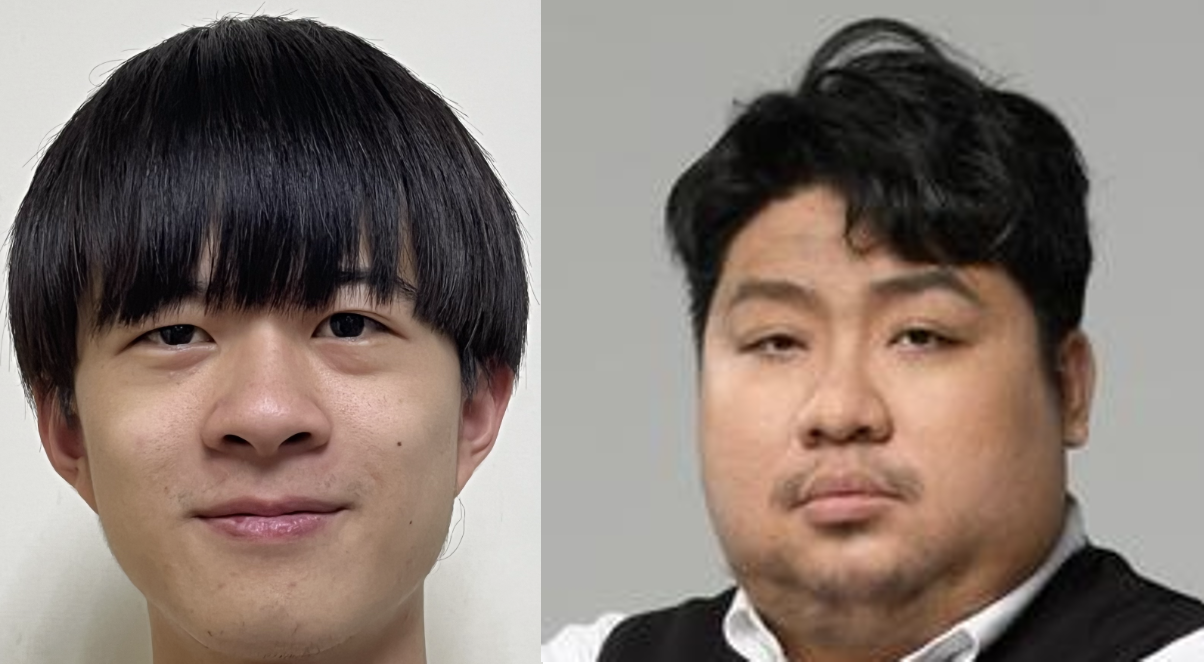
\includegraphics[scale=.25]{fig/source_target_pair.png}
    \caption{left: source image, right: target image}
    \label{fig:source target image}
\end{figure}

\begin{figure}[ht]
\centering
    \centering
    \includegraphics[scale=.05]{fig/change.png}
    \caption{Style fusion between source image and target image, upper left corner is the original reconstructed source image; while lower right corner is the original reconstructed target image}
    \label{fig:stylechange}
\end{figure}

\begin{figure}[ht]
\centering
    \centering
    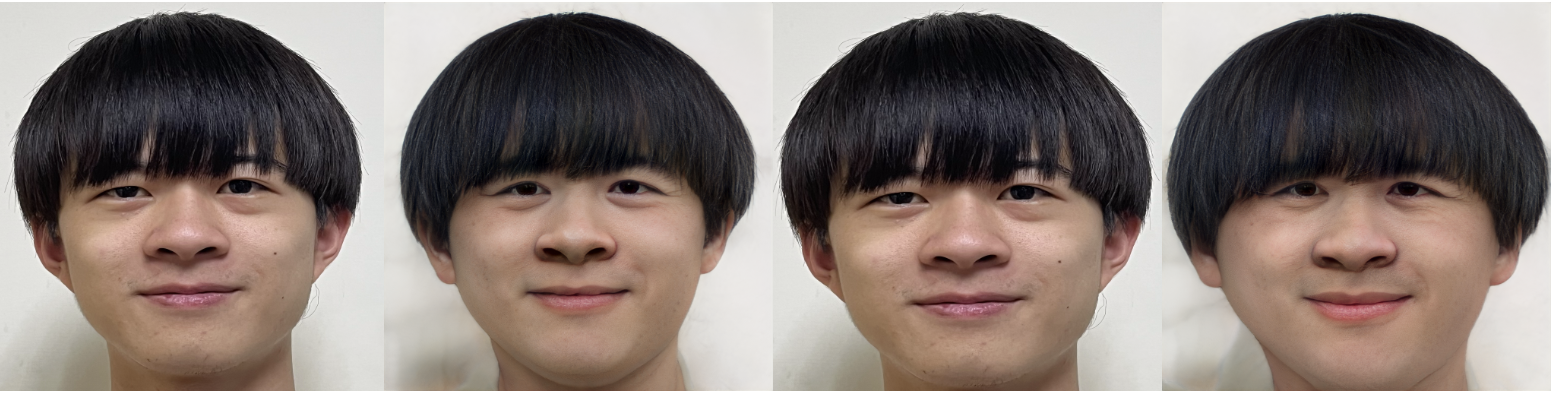
\includegraphics[scale=.3]{fig/cmp_pair.png}
    \caption{face position problem}
    \label{fig:face position problem}
\end{figure}

\subsection{Human Pose Estimation}

The visualization result of human pose is shown in Figure \ref{fig:pose result}.

\begin{figure}[h]
\centering
    \centering
    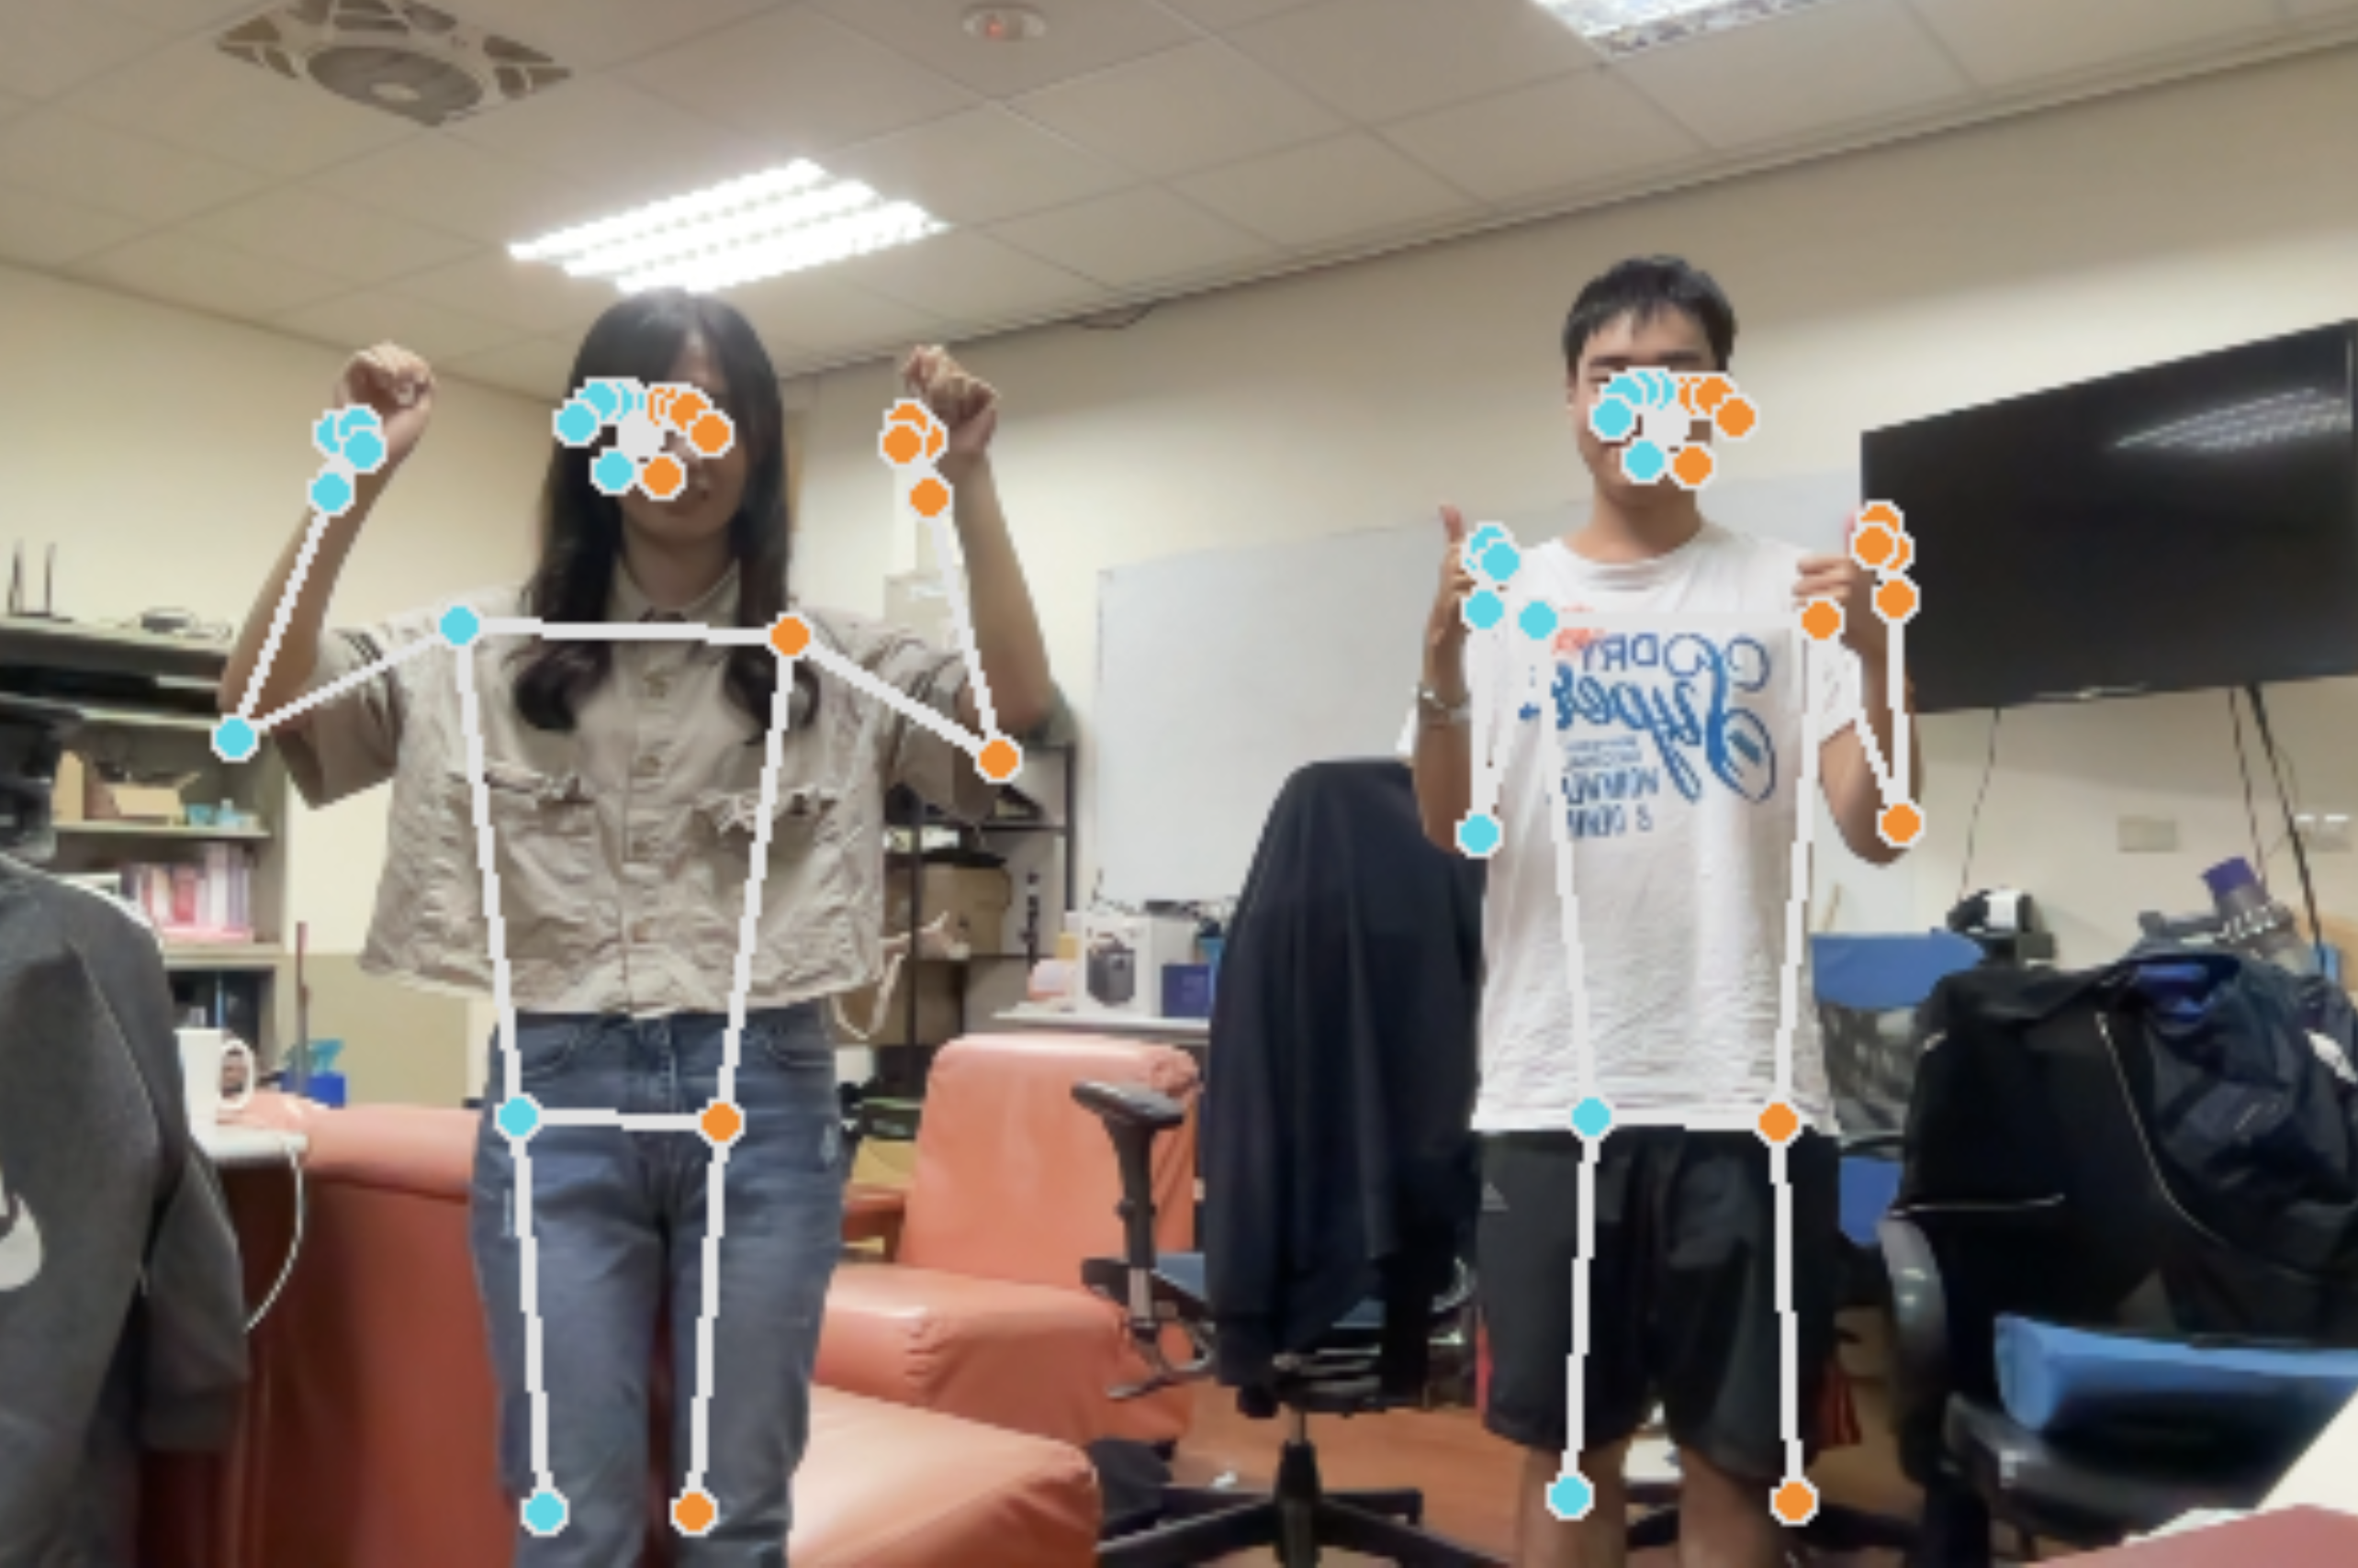
\includegraphics[scale=.15]{fig/pose_result.png}
    \caption{pose result}
    \label{fig:pose result}
\end{figure}
\subsubsection{Implementation Detail}



We conduct an experiment on the accuracy of real-time human pose. There are left person and right person. Each action we do 10 times. 
\subsubsection{Evaluation Metric}
The result is shown in Table \ref{table:eval}. We got an excellent performance in hand raising hand and punching, which achieves 100\% accuracy. As for the last action "hands together", the accuracy is less than other. The main reason is that when we perform this action, the key point position of our hands will get very close, leading to self-occlusion. Under such condition, we observe that the prediction result of mediapipe becomes more unstable, so the average accuracy drops to 75\%.

\begin{table}
\begin{center}
\begin{tabular}{c|c|c|c|c}
\hline
Action & Test Case & \thead{Correct (L)} & \thead{Correct (R)} & \thead{Accuracy  (\%)}\\
\hline 
raise left hand & 10 & 10 & 10 & \textbf{100}\\
% \hline
raise right hand & 10 & 10 & 10& \textbf{100}\\
% \hline
punch left & 10 & 10 & 10 & \textbf{100}\\
% \hline
punch right & 10 & 10 & 10 & \textbf{100}\\
% \hline
hands together & 10 & 8 & 7 & 75 \\
\hline
\end{tabular}
\captionof{table}{Evaluation table for pose2action conversion. \texttt{correct (L)} and \texttt{correct (R)} stands for the number of correctly detected case for left person and right person in the game interface respectively.}
\label{table:eval}
\end{center}
\end{table}
% \begin{center}
% \begin{tabular}{c|c|c|c|c}
% \hline
% Action & test case & \thead{correct (L)} & \thead{correct (R)} & \thead{Accuracy  (\%)}\\
% \hline 
% raise left hand & 10 & 10 & 10 & \textbf{100}\\
% % \hline
% raise right hand & 10 & 10 & 10& \textbf{100}\\
% % \hline
% punch left & 10 & 10 & 10 & \textbf{100}\\
% % \hline
% punch right & 10 & 10 & 10 & \textbf{100}\\
% % \hline
% hands together & 10 & 8 & 7 & 75 \\
% \hline
% \end{tabular}
% \captionof{table}{Evaluation table for pose2action conversion. \texttt{correct (L)} and \texttt{correct (R)} stands for the number of correctly detected case for left person and right person in the game interface respectively.}
% \label{table:eval}
% \end{center}

\subsection{Game Interface}
After integrating with the human pose estimation and StyleGAN, we can use our body motions to control the game character and show the corresponding animation on the screen. Also, when the game character is being attacked, the face of the character will indeed change to the next style image. Finally, we have a live demo on the oral presentation, and the game is working perfectly from it starts to it ends.
\section{Conclusion}
what's the take home message?


% {\small
% \bibliographystyle{ieee_fullname}
% \bibliography{mybib/conference,mybib/others}
% }
{\small
\bibliographystyle{ieee_fullname}
\bibliography{egbib}
}

\end{document}